\section{Naturaleza de los objetivos de aprendizaje}
Un primer conjunto de objetivos de aprendizaje fue propuesto por \cite{Bloom56Taxonomy}. 
Una pequeña variación de la taxonomía de Bloom es resumida a continuación con algunas 
pequeñas adaptaciones al contexto de la computación (utilizando términos como implementar o ejecutar).

En esta discusión se siguen los lineamientos de \cite{Anderson2001Bloom}. 
Tipicamente, un objetivo de aprendizaje contiene un verbo y un pronombre:
El verbo describe el proceso cognitivo que se busca. Luego se incluyen los 
elementos de la taxonomía de Bloom y de esa forma verbos como 
recordar, recordar, entender, analizar, diseñar son altamente relevantes.

Los pronombres describen el conocimiento que se espera que un estudiante adquiera. Luego el conocimiento 
propiamente dicho es categorizado en varias formas en un espectro que va de lo concreto a lo abstracto.

\begin{center}
\begin{table}[h!]
\begin{tabularx}{\textwidth}{|l|l|X|}\hline
\textbf{Nivel} & \textbf{Categoría}      & \textbf{Proceso Cognitivo} \\ \hline
1.     & Recordar 	& reconocimiento, recordar, describir, declarar (\textit{stating}) \\ \hline
2.     & Entender 	& interpretar, ejemplificar, clasificar, inferir, comparar, explicar, parafrasear, resumir \\ \hline
3.     & Aplicar        & ejecutar (i.e. llevar adelante), implementar (i.e. usar), computar, manipular, resolver \\ \hline
4.     & Analizar      	& diferenciar, organizar, atribuir, discriminar, distinguir, sub-dividir \\ \hline 
5.     & Evaluar     	& verificar, criticar, evaluar (\textit{assess}), comparar, contrastar \\ \hline
6.     & Crear       	& generar, planear, producir, innovar, divisar, diseñar, organizar \\ \hline
\end{tabularx}
\label{tab:BloomTaxonomy}
\caption{Taxonomía de Bloom}
\end{table}
\end{center}

Los objetivos del programa tienden a ser asociados con los niveles altos de esta taxonomía. Asi mismo, 
los objetivos instructivos tienden a ser asociados con los niveles bajos de la misma.

\begin{figure}[h!]
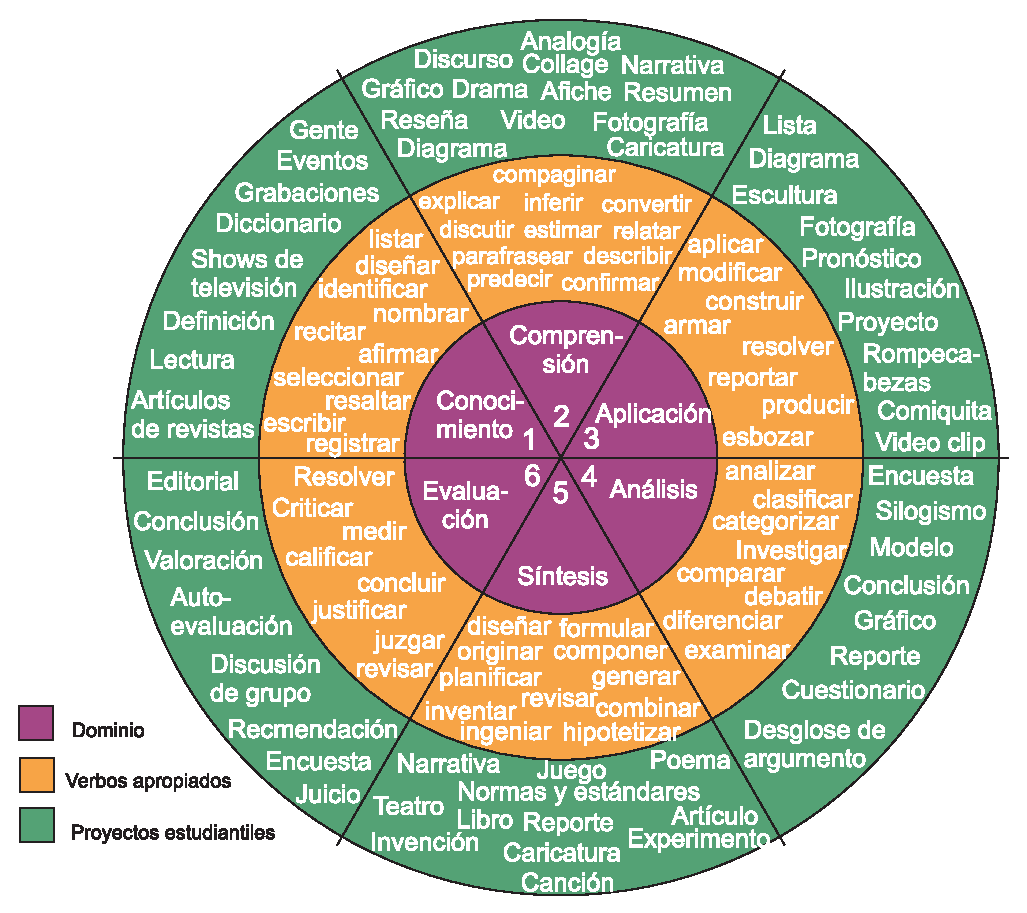
\includegraphics[height=12cm]{\OutputFigDir/Bloom}
\label{fig:BloomTaxonomy}
\caption{Taxonomía de Bloom}
\end{figure} 
